\documentclass[10pt,twocolumn,letterpaper]{article}

\usepackage{cvpr}
\usepackage{times}
\usepackage{epsfig}
\usepackage{graphicx}
\usepackage{amsmath}
\usepackage{amssymb}

% Include other packages here, before hyperref.

% If you comment hyperref and then uncomment it, you should delete
% egpaper.aux before re-running latex.  (Or just hit 'q' on the first latex
% run, let it finish, and you should be clear).
\usepackage[pagebackref=true,breaklinks=true,letterpaper=true,colorlinks,bookmarks=false]{hyperref}

\cvprfinalcopy % *** Uncomment this line for the final submission

\def\cvprPaperID{****} % *** Enter the CVPR Paper ID here
\def\httilde{\mbox{\tt\raisebox{-.5ex}{\symbol{126}}}}

% Pages are numbered in submission mode, and unnumbered in camera-ready
\ifcvprfinal\pagestyle{empty}\fi
\begin{document}

%%%%%%%%% TITLE
\title{An exploration on Wasserstein GAN and a f-GAN}

\author{Chaoqun Jia\\
Department of Computer Science\\
Stanford University\\
{\tt\small enzojia@stanford.edu}
% For a paper whose authors are all at the same institution,
% omit the following lines up until the closing ``}''.
% Additional authors and addresses can be added with ``\and'',
% just like the second author.
% To save space, use either the email address or home page, not both
% \and
% Second Author\\
% Institution2\\
% First line of institution2 address\\
% {\tt\small secondauthor@i2.org}
}

\maketitle
%\thispagestyle{empty}

%%%%%%%%% ABSTRACT
\begin{abstract}
   Generative Adversarial Nets (GAN) provides a straightforward yet effective method for image generation after learning from training data, and researchers have proposed variants under GAN framework. In this project I compare performance of two GAN variants, Wasserstein GAN (WGAN) and $f$-GAN, both of which extend and generalize GAN implementations. Experimental results show that compared to vanilla GAN, WGAN and Pearson $\chi^2$ $f$-GAN have similar capacities on learning data distributions and generating, given features extracted by convolutional networks. This project also explores hyper parameter tuning for WGAN and the results emphasize importance of gradient clipping threshold.
   
\end{abstract}

%%%%%%%%% BODY TEXT
\section{Introduction}

Generative adversarial nets (GAN)\cite{goodfellow2014generative} was proposed as a generative modeling framework in computer vision field. GAN learns probability distributions from training data samples, and accordingly generates new images from random noises. This "learn and generate" mechanism is built on an adversary, with one classifier as the discriminative model to determine whether an image was directly sampled from data or generated by the generator, also another generative component which generates images from random noises. The generator is encouraged by loss function to make the discriminator to classify the generated image as actual data. 

With the essence of generative models being detecting probability densities in existing data, and then generating accordingly, for vanilla GAN and its variants, as discussed in CS231N lectures, the final output of these GANs' discriminators are modeled to be the probability of the input image being an actual image sampled from data and not generated. This is proven to be effective in previous works. However there are other approaches we can consider, and one of them is Wasserstein-GAN (WGAN), which does not train the discriminator (critic) as an classifier outputting probabilities, but only trains it to give scores without the constraint of being between 0 and 1 \cite{arjovsky2017wasserstein}. I will introduce and discuss WGAN in details in the following sections. 

Another way to extend GAN framework is viewing the generator training procedure as minimizing a divergence, which is a variant of Jensen-Shannon divergence, between the model distribution and the real data distribution. After generalizing GAN training procedure from minimizing one specific divergence to minimizing a member of $f$-divergence family, we get $f$-GAN, with the original GAN as a special case for which we train by minimizing a Jensen-Shannon divergence variant, and this variant is a member of $f$-divergence family \cite{nowozin2016fgan}.




\section{Related work}
\label{related_work}

Generative modeling has interested researchers in the past decade. Recent developments include using decoder structures as generators, as by definition decoders are generative and this leads to research efforts of using generalized denoising auto-encoders \cite{bengio2013generalized} as generative models, in which an encoder model was learnt to extract representations and a decoder was learnt to reconstruct the input. An extension from the generalized denoising auto-encoder is deep generative stochastic network (GSN) \cite{bengio2014deep}, as both are developed from the concept of parameterized Markov chain and can be trained by Markov chain Monte Carlo methods (MCMC).

Unlike the Markov chain based generative models mentioned above, GAN was originally introduced by using a minimax loss function, which utilizes results from both a discriminator model and a generator model \cite{goodfellow2014generative}. With the goal being replicating the data probability distribution, this minimax loss function is adopted to reflect the distance between the distribution of real data versus the distribution of the generated data. As described by the original research, vanilla GAN structure treats its discriminator output as the probability of the input being sampled from real data. Meanwhile there are other approaches which do not restrict the discriminator output to be a probability, being less than 1 and greater than 0. One example of these approaches is Wasserstein-GAN (WGAN) that minimizes an approximation of Earth Mover (EM) distance, as this approximation is proven to be reasonable and efficient \cite{arjovsky2017wasserstein}.

As discussed in the original GAN paper, there is another perspective which sees training GAN as minimizing a variant of Jensen-Shannon divergence. S. Nowozin et.al \cite{nowozin2016fgan} pushes this idea further to generalize training objectives of GAN to the whole $f$-divergence family, and corresponding GAN variant is named $f$-GAN. Examples of $f$-divergence family discussed in the original $f$-GAN paper include Kullback-Leibler divergence, Reverse KL divergence, Pearson $\chi^2$ divergence, Squared Hellinger divergence, Jensen-Shannon divergence, and the GAN divergence which is derived from Jensen-Shannon. The authors proved the soundness of this generalization both in theory and in empirical results. Further experiments are conducted under a setting of using different divergences in $f$-divergence family for train and test, respectively, and test loss values are calculated and compared. Results show that even trained with a different divergence in the family, the test loss values are still reasonably low, and the best performance comes from using the same divergence for train and test. 



\section{Data}
\label{data}

\subsection{Actual image data}
\label{actual_image}
The MNIST (Modified National Institute of Standards and Technology) database is a large database containing 60000 training images and 10000 testing images to be used for training computer vision models \cite{mnist}. This dataset was originally created by NIST, with the training set was taken from a handwritten sample by U.S. Census Bureau employees, and the testing set was taken from U.S. high school students. The difference in sources for training versus testing sets makes it arguable whether NIST database is a good dataset for training machine learning models. So the authors applied a "re-mixing" to the NIST database and the output is MNIST database, with data points from both sources evenly distributed to both training and testing sets. With this remix strategy, MNIST collects more diversified handwriting styles and keeps consistent patterns. Authors of this database used support vector machine to achieve a higher than 99\% recognition accuracy \cite{726791}. In this project I only use the training set of MNIST data, from which my strategy randomly select 50000 images for model training and 5000 for model validation. 

Each data point of MNIST database is an image of a handwritten digit, has only one channel because each image is black and white so there is a grey-scale channel, also the images are normalized to fit into a 28 by 28 pixel resolution.


\subsection{Noise generation}
\label{noise}
For a GAN's generator model to start with, we need noise input as seed to generate new images. In this project I use a uniform pseudo-random noise with values between -1 and 1. The noise generation directly outputs a noise matrix with dimension of batch size by noise size, and each element of this matrix is independent to all other elements. Noise size is aligned with generator model's input size so we can use it as a seed. 


\section{Methods}
\label{methods}
\subsection{Vanilla GAN}
\label{vanilla_gan}

The original GAN design provides a framework to include two component models:
\begin{itemize}
    \item A generator model $G(z; \theta_g)$ which takes a random noise vector of an arbitrary size as input seed, and generates an image by sampling from the probability distributions learnt from training dataset. 
    \item A discriminator model which is a classifier $D(x;\theta_d)$. It takes an image as input and outputs a scalar as classification result, indicating whether this image is genuine from real data or is generated by the generator $G(z; \theta_g)$.
\end{itemize}

In other words, $G(z; \theta_g)$ is a mapping from input noise vectors to data space, parameterized by $\theta_g$, and $z$ is the input noise which has a prior distribution $p_z(z)$. We usually design $G$ to be a differentiable function so we can learn the generator's distribution $p_g$ over data $x$ by applying gradient descent/ascent optimizers. Meanwhile discriminator $D(x;\theta_d)$ is parameterized by $\theta_d$ and its scalar output is usually interpreted as the probability that the input $x$ is sampled from data rather than generated by $G$. Goal of training of a GAN is to have D to maximize the probability of correctly labeling an input image whether it is from actual data or generated by G, and meanwhile to have G to minimize the probability that D labels generated images correctly. To achieve this goal the authors developed the minimax loss function as shown in equation \ref{loss_gan}.

\begin{equation} 
\begin{split}
\begin{aligned}
\underset{G}{\text{min}}\; \underset{D}{\text{max}}\; \mathbb{E}_{x \sim p_\text{data}}\left[\log D(x)\right] + \mathbb{E}_{z \sim p(z)}\left[\log \left(1-D(G(z))\right)\right]
\end{aligned}
\end{split}
\label{loss_gan}
\end{equation}

Goodfellow et al. \cite{goodfellow2014generative} proved that given G and D are parameterized to have enough capacity, the training criterion in equation \ref{loss_gan} makes it possible to recover the data distribution. In actual implementations of this loss function we update the discriminator and generator alternatively, as shown in Algorithm 1 in page 8, which is proven to optimize the loss function as demonstrated by equation \ref{loss_gan}.

\subsection{Wasserstein GAN}
\label{wasserstein_gan}

An usual approach to learn the probability distribution in training data is equivalent to solving:

\begin{equation} 
\begin{split}
\begin{aligned}
\underset{\theta \in R^d}{\text{max}} \frac{1}{m} \Sigma_{i=1}^m \log \mathbb{P}_{\theta}(x^{(i)})
\end{aligned}
\end{split}
\label{loss_gan_ii}
\end{equation}

where $x^{(i)}$ are examples from training data. This approach uses model density $\mathbb{P}_\theta$ to approximate the real data distribution $\mathbb{P}_r$ and minimizes the Kullback-Leibler divergence $KL(\mathbb{P}_r||\mathbb{P}_\theta)$. In the Wasserstein GAN (WGAN) method which was proposed by M. Arjovsky et. al \cite{arjovsky2017wasserstein}, the authors use Earth-Mover distance which is also know as Wasserstein-1, to measure the distance between model distribution and real data distribution. As proven by the authors, the Earth-Mover distance provide similar properties compared to other probability distances and divergences, including Total Variance (TV) distance, Kullback-Leibler (KL) divergence, and Jensen-Shannon (JS) divergence. With Earth-Mover distance defined as equation \ref{em_i}.

\begin{equation} 
\begin{split}
\begin{aligned}
W(\mathbb{P}_r, \mathbb{P}_g) = \underset{\gamma \in \Pi(\mathbb{P}_r, \mathbb{P}_g)}{\text{inf}} \mathbb{E}_{(x, y) \sim\gamma}[||x - y||]
\end{aligned}
\end{split}
\label{em_i}
\end{equation}

where $\Pi(\mathbb{P}_r, \mathbb{P}_g)$ denotes the set of all joint distributions $\gamma(x, y)$ whose marginals are respectively $\mathbb{P}_r$ and $\mathbb{P}_g$. In practice we do not use the distance defined in equation \ref{em_i} because it is intractable, however according to Kantorovich-Rubinstein duality we have equation \ref{em_ii}.


\begin{equation} 
\begin{split}
\begin{aligned}
W(\mathbb{P}_r, \mathbb{P}_\theta) = \underset{||f||_L \le 1}{\text{sup}} \mathbb{E}_{x \sim\mathbb{P}_r}[f(x)] -  \mathbb{E}_{x \sim\mathbb{P}_\theta}[f(x)]
\end{aligned}
\end{split}
\label{em_ii}
\end{equation}

where function $f$ for the supremum is any 1-Lipschitz function mapping from domain to $\mathbb{R}$. In the original paper for WGAN the authors prove existence of a solution $f: \mathcal{X} \xrightarrow{} \mathbb{R}$ to the optimization problem \ref{em_ii}, and we can calculate corresponding gradient by applying:

\begin{equation} 
\begin{split}
\begin{aligned}
\nabla_{\theta} W(\mathbb{P}_r, \mathbb{P}_\theta) = - \mathbb{E}_{z \sim p(z)}[\nabla_{\theta}f_w(g_\theta(z))] 
\end{aligned}
\end{split}
\label{em_gradient}
\end{equation}

where $\mathbb{P}_\theta$ is the distribution of $g_\theta(z))$ and with $Z$ being a random variable with density $p$ satisfying the assumption discussed by equation \ref{em_i}. Now we have gradient of the model's parameters and can work on the algorithm, as shown in algorithm 2 in page 8. To keep terms consistent with the original paper, here we name $f_w$ as critic and $g_\theta$ as generator. In WGAN's algorithm 2 there are parts I highlight in blue, and these blue lines are differences between training algorithms of WGAN versus GAN. From this comparison we can see the main difference lies in the loss function, and the root reason of the loss functions being different is that in GAN we assume the discriminator (critic) outputs a probability of the input image being real data, however in WGAN we do not have this assumption. Thus WGAN's critic's output is not restricted to be between 0 and 1, so there is not a threshold to determine whether an input image is real or generated. Under this setting, design of loss function just encourages the critic (discriminator) to make the output scalar bigger for real input images and smaller for generated ones.






\subsection{f-GAN}
\label{f_gan}

In the original paper for vanilla GAN \cite{goodfellow2014generative} the authors recognize that one perspective to see training procedure of the generator is minimizing a variant of the Jensen-Shannon divergence between the model distribution and the real data distribution:

\begin{equation} 
\begin{split}
\begin{aligned}
D_{JS}(p_{data}||p_g) = &\frac{1}{2} D_{KL}(p_{data}||\frac{p_{data} + p_g}{2}) \\
&+ \frac{1}{2} D_{KL}(p_g||\frac{p_{data} + p_g}{2})
\end{aligned}
\end{split}
\label{d_js}
\end{equation}

where $p_g$ is the generator's distribution, and $p_{data}$ is real data's true distribution, and $D_{KL}$ is Kullback-Leibler divergence. In the work by S. Nowozin et.al \cite{nowozin2016fgan} the authors propose a training method which generalize the Jensen-Shannon divergence discussed above to $f$-divergence family, also known as Ali-Silvey distances. 

\begin{equation} 
\begin{split}
\begin{aligned}
    D_f(P||Q) = \int_{\mathcal{X}} q(x) f\left(\frac{p(x)}{q(x)}\right) dx 
\end{aligned}
\end{split}
\label{f_divergence}
\end{equation}

where P and Q are two distributions with continuous density functions p and q respectively, and $\mathcal{X}$ is the domain for p and q. $f: \mathbb{R_+} \xrightarrow{} \mathbb{R}$ is the generator function which is convex and lower-semicontinuous, and $f(1) = 1$. The original $f$-GAN paper provides a list of common choices of $f$-divergences, and here I list two of them, Pearson $\chi^2$ divergence which I used in my experiments, and GAN divergence, which is derived from Jensen-Shannon divergence, for the purpose of demonstration. Both Pearson $\chi^2$ and GAN divergences are listed in table \ref{f_divergence_examples}, with a function $T^*$ derived as 
\begin{equation} 
\begin{split}
\begin{aligned}
    T^* =  f'\left(\frac{p(x)}{q(x)}\right) dx 
\end{aligned}
\end{split}
\label{f_divergence}
\end{equation}


The original $f$-GAN paper proved validness of equation \ref{f_divergence_obj} as a loss function, which can be calculated using the $f$-divergence definitions in table \ref{f_divergence_examples}

\begin{equation} 
\begin{split}
\begin{aligned}
    \underset{\theta}{\text{min}}\; \underset{w}{\text{max}} \; \mathbb{E}_{x\sim P} [T_w(x)] - \mathbb{E}_{x\sim Q_\theta} [f^*(T_w(x))]
\end{aligned}
\end{split}
\label{f_divergence_obj}
\end{equation}

where $Q_\theta$ is the generative model parameterized by $\theta$ and $T_w$ is the discriminator, named "variational function" in the $f$-GAN paper, parameterized by w. We assume this variational function $T_w$ is represented as $g_f(V_w(x))$, and can rewrite the loss function as:

\begin{equation} 
\begin{split}
\begin{aligned}
    \underset{\theta}{\text{min}}\; \underset{w}{\text{max}} \; \mathbb{E}_{x\sim P} [g_f(V_w(x))] + \mathbb{E}_{x\sim Q_\theta} [-f^*(g_f(V_w(x)))]
\end{aligned}
\end{split}
\label{f_divergence_obj_ii}
\end{equation}
where $V_w: \mathcal{X} \xrightarrow{} \mathbb{R}$ is implemented with a neural network, and $g_f: \mathbb{R} \xrightarrow{} dom_{f^*}$ is an output activation function. Table \ref{f_divergence_functions} provides $V_w$ and $g_f$ for Pearson $\chi^2$ and GAN divergences, as provided arbitrarily in the original $f$-GAN paper, and after filling $V_w$ and $g_f$ for Pearson $\chi^2$ into equation \ref{f_divergence_obj_ii} we get $f$-GAN algorithm 3 in page 9. In this algorithm illustration there are parts I highlight in red, and these red lines are differences between training algorithms of $f$-GAN versus GAN. From this comparison we can see the main difference lies in the loss function, plus activation function for each neural network. In my experiment I used Pearson $\chi^2$ as an example to demonstrate implementations of $f$-divergences other than Jensen-Shannon divergence, and this choice leads to different loss functions and different final-layer activations for both generator and discriminator.  


\begin{table*}[t]
  \centering
  \begin{tabular}{llll}
 Name & $D_f(P||Q)$ & Generator $f(u)$ & $T^*(x)$ \\ \hline
 Pearson $\Chi^2$ & \int \frac{(q(x) - p(x))^2}{p(x)}dx & $(u-1)^2$ & 2\left(\frac{p(x)}{q(x)} - 1\right) \\
 GAN & \int p(x)\log \frac{2p(x)}{p(x) + q(x)} + q(x) \log \frac{2q(x)}{p(x) + q(x)} dx -\log(4) & u\log(u) - (u + 1) \log(u + 1) & \log \frac{p(x)}{p(x) + q(x)} \\ \hline
  \end{tabular}
  \caption{ Pearson $\Chi^2$ and GAN $f$-divergences $D_f(P||Q)$ and corresponding generator functions. GAN is derived from Jensen-Shannon divergence as $D_{GAN} = 2D_{JS} - \log(4)$. }
  \label{f_divergence_examples}
\end{table*}


\begin{table*}[t]
  \centering
  \begin{tabular}{llll}
 Name & Output activation $g_f$ & dom_{f^*}  & Conjugate $f^*$ \\ \hline
 Pearson $\Chi^2$ & v & $\mathbb{R}$ & $\frac{1}{4} t^2 + t$ \\
 GAN & -\log (1 + exp(-v)) & $\mathbb{R}_\_$ & -\log (1 - \exp (t))  \\ \hline
  \end{tabular}
  \caption{Final layer activation functions, conjugate $f^*$ and corresponding domain, for Pearson $\Chi^2$ and GAN $f$-divergences.}
  \label{f_divergence_functions}
\end{table*}



% \begin{table*}[t]
%   \centering
%   \begin{tabular}{lcr}
%    {\bf Algorithm 1} GAN. k is number of steps to apply to the discriminator. \\
%    {\color{black} In the original paper k = 1.}\\ \hline
%    {\bf for} number of training iterations {\bf do}\\
%    \hspace{4mm} {\bf for} k steps {\bf do}\\
%    \hspace{8mm} Sample minibatch of $m$ noise samples ${z^{(1)}, ..., z^{(m)}}$ from noise prior $p_g(z)$\\
%    % $p_g(z)$\\
%    \hspace{8mm} Sample minibatch of $m$ image samples ${x^{(1)}, ..., x^{(m)}}$ from data generating distribution $\mathbb{P}_r(x)$\\
%    \hspace{8mm} Update the discriminator with chosen optimizer using gradient: \\
%    \hspace{16mm} $\nabla_{\theta_d} \frac{1}{m} \Sigma_{i=1}^m [\log D(x^{(i)}) + \log (1 - D(G(z^{(i)})))]$ \\
%    \hspace{4mm} {\bf end for} \\
%    \hspace{4mm} Sample minibatch of $m$ noise samples ${z^{(1)}, ..., z^{(m)}}$ from noise prior $p_g(z)$\\
%    \hspace{4mm} Update the discriminator with chosen optimizer using gradient: \\
%    \hspace{16mm} $\nabla_{\theta_g} \frac{1}{m} \Sigma_{i=1}^m \log (1 - D(G(z^{(i)})))$ \\   
%    {\bf end for} \\ \hline
%   \end{tabular}
%   \label{algo_gan}
% \end{table*}


% \begin{table*}[t]
%   \centering
%   \begin{tabular}{lcr}
%    {\bf Algorithm 2} WGAN. k is number of steps to apply to the discriminator and c is weight clipping threshold. \\
%    {\color{blue} In the original paper k = 5 and c = 0.01.} \\ \hline
%    {\bf for} number of training iterations {\bf do}\\
%    \hspace{4mm} {\bf for} k steps {\bf do}\\
%    \hspace{8mm} Sample minibatch of $m$ noise samples ${z^{(1)}, ..., z^{(m)}}$ from noise prior $p_g(z)$\\
%    \hspace{8mm} Sample minibatch of $m$ image samples ${x^{(1)}, ..., x^{(m)}}$ from data generating distribution $\mathbb{P}_r(x)$\\
%    % $p_{data}(x)$\\
%    \hspace{8mm} Update the discriminator with chosen optimizer using gradient: \\
%    \hspace{16mm} {\color{blue} $\nabla_{w} [\frac{1}{m} \Sigma_{i=1}^m f_w(x^{(i)}) + \frac{1}{m} \Sigma_{i=1}^m  f_w(g_\theta(z^{(i)}))]$} \\
%    \hspace{16mm} {\color{blue} w $\xleftarrow{}$ clip(w, -c, c)}\\
%    \hspace{4mm} {\bf end for} \\
%    \hspace{4mm} Sample minibatch of $m$ noise samples ${z^{(1)}, ..., z^{(m)}}$ from noise prior $p_g(z)$\\
%    \hspace{4mm} Update the discriminator with chosen optimizer using gradient: \\
%    \hspace{16mm} {\color{blue} $\nabla_{\theta} \frac{1}{m} \Sigma_{i=1}^m f_w(g_\theta(z^{(i)}))$ }\\   
%    {\bf end for} \\ \hline
%   \end{tabular}
%   \label{algo_wgan}
% \end{table*}


% \begin{table*}[t]
%   \centering
%   \begin{tabular}{lcr}
%    {\bf Algorithm 2} $f$-GAN. k is number of steps to apply to the discriminator. \\
%    {\color{black} In the original paper k = 1.} \\ \hline
%    {\bf for} number of training iterations {\bf do}\\
%    \hspace{4mm} {\bf for} k steps {\bf do}\\
%    \hspace{8mm} Sample minibatch of $m$ noise samples ${z^{(1)}, ..., z^{(m)}}$ from noise prior $p_g(z)$\\
%    \hspace{8mm} Sample minibatch of $m$ image samples ${x^{(1)}, ..., x^{(m)}}$ from data generating distribution $\mathbb{P}_r(x)$\\
%    % $p_{data}(x)$\\
%    \hspace{8mm} {\color{red} Apply $g_f$ as final layer activation function. For Pearson $\Chi^2$ it is identical function.} \\
%    \hspace{8mm} Update the discriminator with chosen optimizer using gradient: \\
%    \hspace{16mm} {\color{red} $\nabla_{w} [\frac{1}{m} \Sigma_{i=1}^m g_f(V_w(x^{(i)})) - \frac{1}{m} \Sigma_{i=1}^m f^*(g_f(V_w(z^{(i)})))]$, which for Pearson $\Chi^2$ is:}\\
%    \hspace{16mm} {\color{red} $\nabla_{w} [\frac{1}{m} \Sigma_{i=1}^m V_w(x^{(i)}) + \frac{1}{m} \Sigma_{i=1}^m \left( \frac{1}{4} V_w(z^{(i)})^2 + V_w(z^{(i)})\right)]$}\\
%    % \hspace{16mm} {\color{blue} w $\xleftarrow{}$ clip(w, -c, c)}\\
%    \hspace{4mm} {\bf end for} \\
%    \hspace{4mm} Sample minibatch of $m$ noise samples ${z^{(1)}, ..., z^{(m)}}$ from noise prior $p_g(z)$\\
%    \hspace{4mm} Update the discriminator with chosen optimizer using gradient: \\
%    \hspace{16mm} {\color{red} $\nabla_{w} [\frac{1}{m} \Sigma_{i=1}^m f^*(g_f(V_w(z^{(i)})))]$, which for Pearson $\Chi^2$ is:}\\
%    \hspace{16mm} {\color{red} $\nabla_{w} [ - \frac{1}{m} \Sigma_{i=1}^m \left( \frac{1}{4} V_w(z^{(i)})^2 + V_w(z^{(i)})\right)]$}\\
%    % \hspace{16mm} {\color{blue} w $\xleftarrow{}$ clip(w, -c, c)}\\  
%    {\bf end for} \\ \hline
%   \end{tabular}
%   \label{algo_fgan}
% \end{table*}


\section{Experiment results}
\label{experiments}

\subsection{Experimental settings}
\label{exp_settings}
As the purpose of this experiment is to compare image generation qualities by vanilla GAN, WGAN, and $f$-GAN, I implemented corresponding algorithms as described in Algorithms 1, 2, and 3 in page 8 and 9. For $f$-GAN I choose Pearson $\chi^2$ divergence as the optimization goal. Meanwhile I also test two different designs for generator / discriminator (critic) networks, one with only fully connected layers and the other design with convolutional layers. So there are 6 training-testing runs, for 3 types of GANs and each type has two different generator/discriminator network designs. In this design of experiment settings I achieve comparison on two dimensions:
\begin{itemize}
    \item Performance differences in image generation qualities, between GAN, WGAN, and Pearson $\chi^2$ $f$-GAN.
    \item Performance differences in feature extraction qualities, between pure fully-connected networks and convolutional networks.
\end{itemize}

For the fully-connected networks and convolutional networks, I reuse the network designs used in GAN part of CS231N assignment 3, as these network designs are proven to work, and my focus in this project is not designing these networks but on comparing vanilla GAN versus WGAN versus $f$-GAN architectures. 

\subsection{Metrics}
\label{metrics}
For handwritten digit image generation there is no good quantified metric to measure generation quality, as human handwriting styles is not easy to quantify. However during experiments I found that by putting generated images side by side we can use human intuition to determine which one is better. For the ones with lower qualities they usually have observable flaws, e.g. written stokes are distorted too much from human writing habits, etc. These observable flaws make it possible to use human judgement as image generation quality measurement.


\subsection{Hyper parameters}
\label{hyper_parameters}
Other than usual network training hyper parameters including learning rate, batch size etc., in the original paper for Wasserstein GAN (WGAN) the authors discussed about one hyper parameter which is weight clipping threshold, for the purpose of enforcing a Lipschitz constraint. Also during my own experiment I introduced another hyper parameter which is gradient clipping threshold, and this makes WGAN having two non-usual hyper parameters.

\subsection{Results and discussions}
\label{results}
\subsubsection{Comparison between GAN variants}
\label{gan_variants}
In figure \ref{gans_conv} I compare generated digit images by vanilla GAN in first row, WGAN in second row, and $f$-GAN in third row, respectively. Also images in the left column are generated using features extracted by fully connected layers, and images in the right column are generated using features extracted by convolutional network. 
\begin{itemize}
    \item To compare vanilla GAN vs. WGAN vs. $f$-GAN using features extracted by fully-connected layers, WGAN and $f$-GAN's performance are not comparable to vanilla GAN, as only vanilla GAN generates recognizable digits, though the digit images are of low quality with scattering noises.
    \item Vanilla GAN vs. WGAN vs. $f$-GAN using features extracted by convolutional networks generate digit images of similar qualities, while I observe that Pearson $\chi^2$ $f$-GAN generates with arguably better quality because its handwriting style aligns better with human handwriting habits. Most generated digits are readable, with small numbers of them being distorted. Meanwhile these three GAN variants' generations have recognizable different styles, for example WGAN's digit images have thicker strokes.
    \item Fully connected layers vs. convolutional networks. We can observe that convolutional networks extract higher-quality image features, because for each GAN variant it performs better using features extracted by convolutional networks.
\end{itemize}

\subsubsection{WGAN hyper parameter tuning}
\label{wgan_hyper_parameter_tuning}

In figure \ref{gans_conv_hyper_p} I focus on WGAN's performance under different hyper parameter settings. Each row corresponds to one gradient clipping threshold value, and each column corresponds to one weight clipping threshold value. One observation not reflected in the figures is that for the one setting with no gradient clipping and no weight clipping, I observed exploding network weights causing loss to the level of $1e6$, and the generated images are not stable and much distorted. The final result of my hyper parameter search is using gradient clipping threshold at $7.5e-8$ and weight clipping threshold at 0.001 which is the same as the original WGAN paper suggested. 

\begin{itemize}
    \item On weight clipping threshold dimension, we can observe that if the value is too small (0.00001) than we only see noise caused by vanishing gradients because too many weights are clipped. Meanwhile if the values is too large (0.1) the result is not stable. 
    \item On gradient clipping threshold dimension, we have similar conclusion that too small clipping threshold ($1e-10$) has a high probability to cause vanishing gradient thus more random noisy images, and too large clipping threshold ($1e-5$) makes the network unstable and thus generates more distorted digits.
\end{itemize}

Also looking at the degree of distortion in subplots (a), (b), (d), and (e) in figure \ref{gans_conv_hyper_p}, as for these 4 plots both clipping thresholds are not extremely small to cause vanishing gradient, my observation is that gradient clipping threshold has a bigger impact on the generator performance, as both plots (d) and (e) are better formed compared to (a) and (b) respectively. 





\section{Conclusions}
\label{conclusions}
In this project I implement WGAN and Pearson $\chi^2$ $f$-GAN, and compare images generated by them versus vanilla GAN. Two types of generator / discriminator (critic) networks are implemented, one with only fully-connected layers and the other with convolutional layers. To conclude this project, the experimental results prove that under help of features extracted by convolutional layers, both WGAN and Pearson $\chi^2$ $f$-GAN generate images with qualities comparable to vanilla GAN, and Pearson $\chi^2$ $f$-GAN's generation has slight better performance in some dimensions including mimicking human handwriting styles. 

There are other observations not directly from comparing different types of GANs, including: 1) convolutional neural networks provide significantly better features for image learning and generating, compared to fully-connected networks, and 2) WGAN has more hyper parameters to tune, and it is sensitive to weight and gradient clipping thresholds, especially to gradient clipping threshold.

\section{Future works}
\label{future_works}

In my experiments I have one observation for WGAN hyper parameter which is not aligned with the observation in the original WGAN paper, that the original paper emphasizes importance of weight clipping and does not mention gradient clipping, however in my experiments I find that given weight clipping threshold is not extremely small, gradient clipping has larger impact on WGAN's generation quality. There are multiple possibilities causing the differences in tuning methods, including differences in building generator and critic, and interactions between weight and gradient clipping thresholds, etc. In the future I will work on more experiments on the possibilities mentioned above and try to resolve this non-alignment.

\section{Contributions and acknowledgements}
\label{acknowledgements}

This is a one-person project for CS231N, all experiments and documentation are completed by the sole author himself. This project is not shared by any other class, and there is no non-CS231N external collaborators. Python code for the experiments are developed based on CS231N assignment 3 code, with re-written ipynb notebooks, re-written GAN training methods, and new loss function methods. Data pre-processing code and generator/discrimnator network designs are re-used.

\begin{figure*}
\centering
\begin{tabular}{cc}
  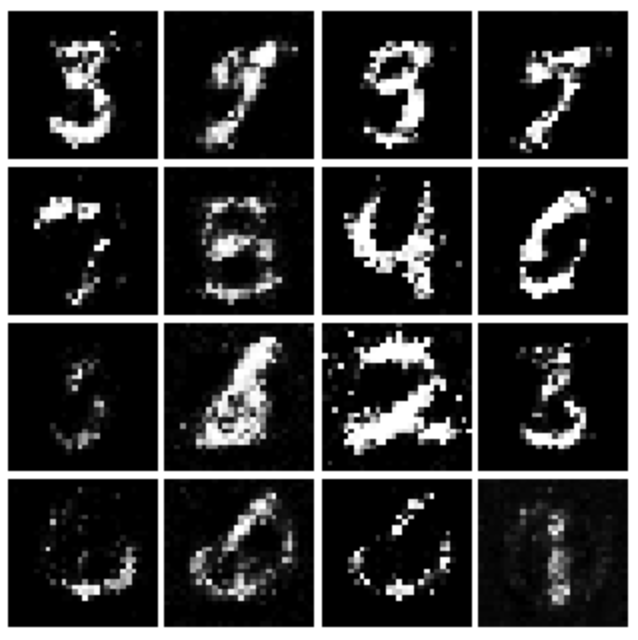
\includegraphics[width=65mm]{latex/GAN_noConv.png} &   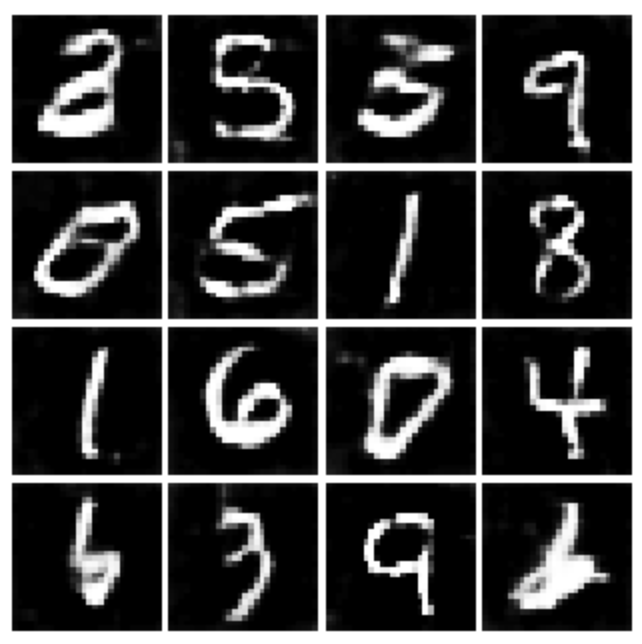
\includegraphics[width=65mm]{latex/GAN_Conv.png} \\
(a) Vanilla GAN without Conv layers & (b) Vanilla GAN with Conv layers \\[6pt]
 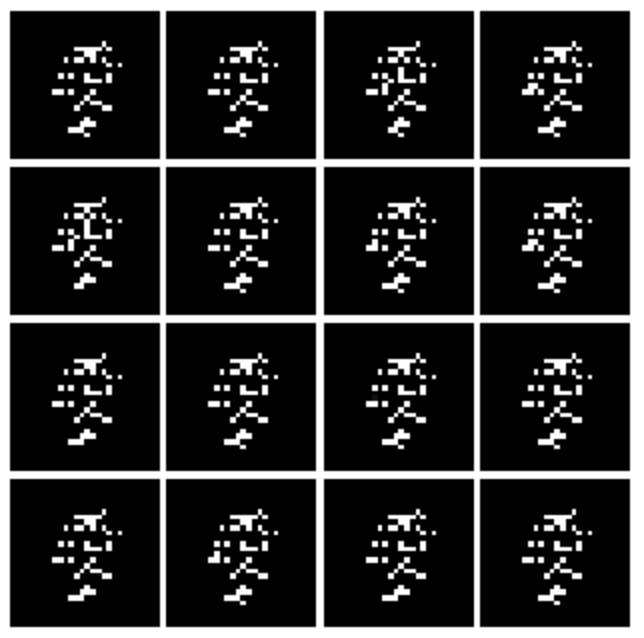
\includegraphics[width=65mm]{latex/WGAN_noConv.png} &   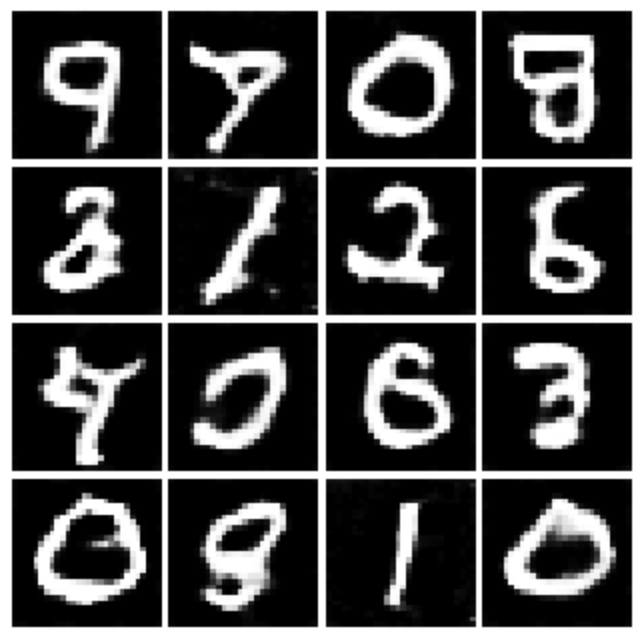
\includegraphics[width=65mm]{latex/WGAN_Conv.png} \\
(c) WGAN without Conv layers & (d)WGAN with Conv layers \\[6pt]
 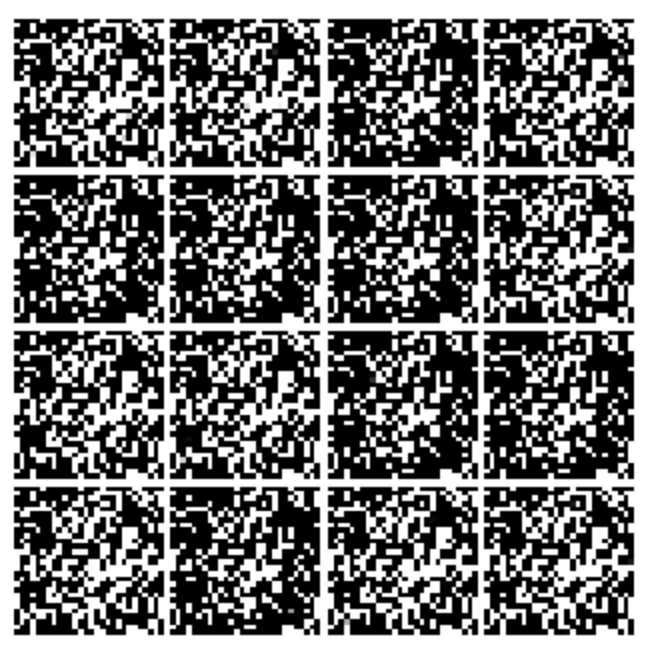
\includegraphics[width=65mm]{latex/fGAN_noConv.png} &   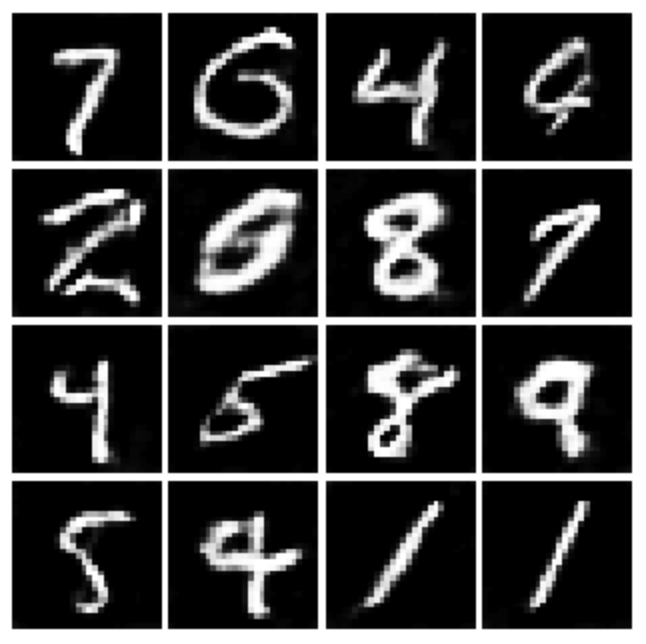
\includegraphics[width=65mm]{latex/fGAN_Conv.png} \\
(c) $f$-GAN without Conv layers & (d) $f$-GAN with Conv layers \\[6pt]
\end{tabular}
\caption{Digit images generated by Vanilla GAN, WGAN, and $f$-GAN, with and without Convolution layers for feature extractions, respectively.}
\label{gans_conv}
\end{figure*}

\begin{figure*}
\centering
\begin{tabular}{ccc}
  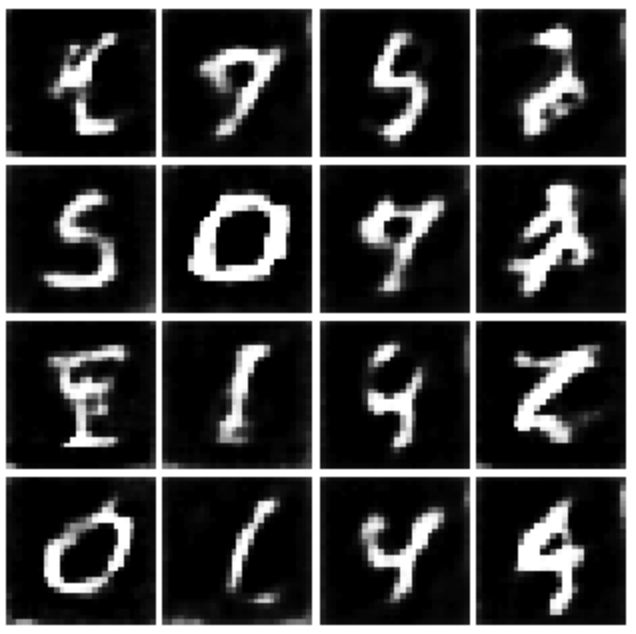
\includegraphics[width=44mm]{latex/WGAN_1e_n5_p1.png} &   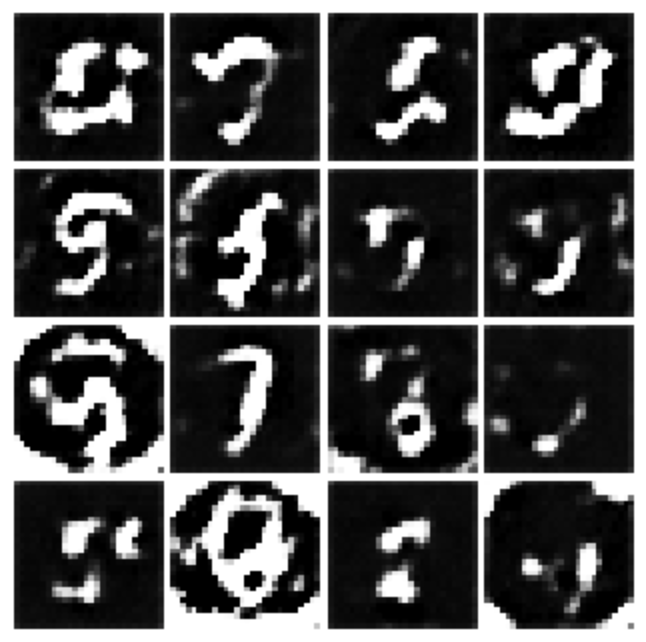
\includegraphics[width=44mm]{latex/WGAN_1e_n5_p001.png} &   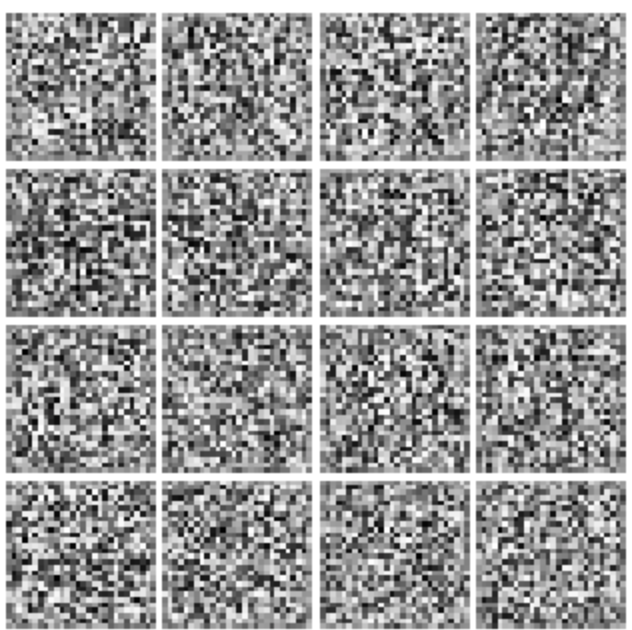
\includegraphics[width=44mm]{latex/WGAN_1e_n5_p00001.png} \\
(a) gradient threshold: $1e-5$ & (b)  gradient threshold: $1e-5$ & (c)  gradient threshold: $1e-5$\\[6pt]
(a) weight threshold: 0.1 & (b) weight threshold: 0.001 & (c)  weight threshold: 0.00001\\[6pt]
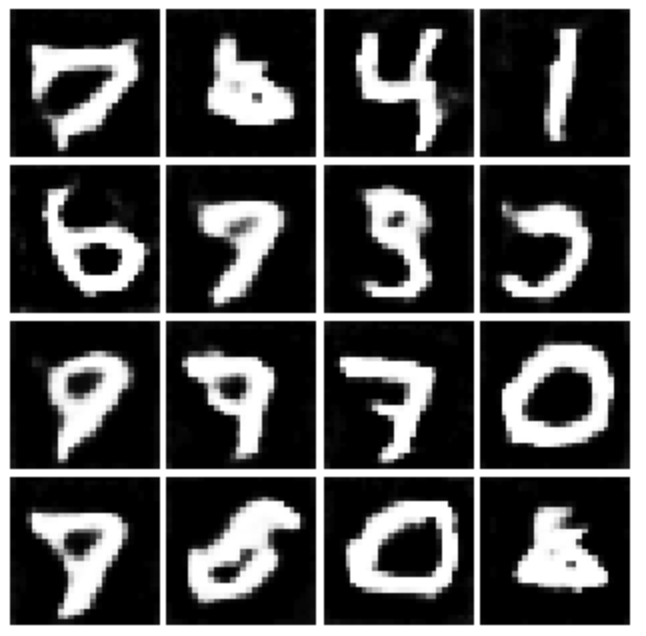
\includegraphics[width=44mm]{latex/WGAN_7p5e_n8_p1.png} &   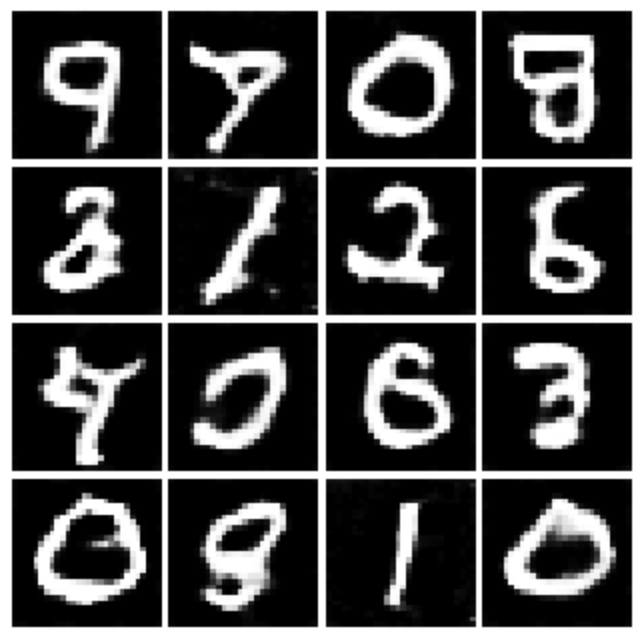
\includegraphics[width=44mm]{latex/WGAN_7p5e_n8_p001.png} &   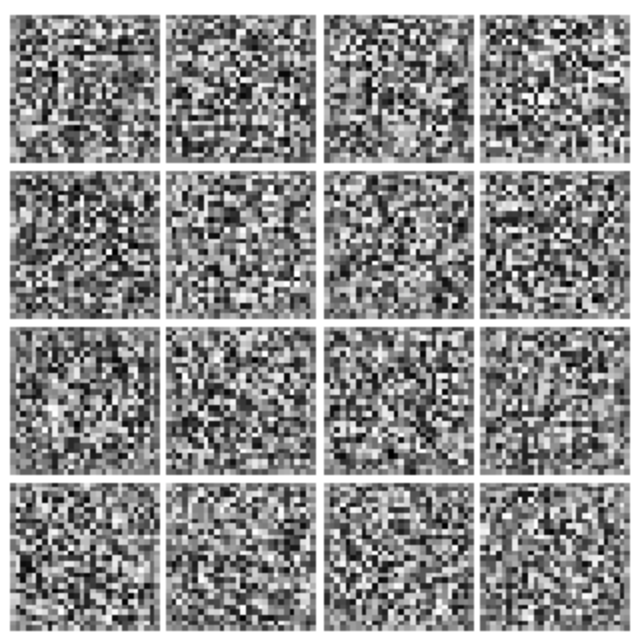
\includegraphics[width=44mm]{latex/WGAN_7p5e_n8_p00001.png} \\
(d) gradient threshold: $7.5e-8$ & (e)  gradient threshold: $7.5e-8$& (f)  gradient threshold: $7.5e-8$\\[6pt]
(d)weight threshold: 0.1 & (e)weight threshold: 0.001 & (f)  weight threshold: 0.00001\\[6pt]
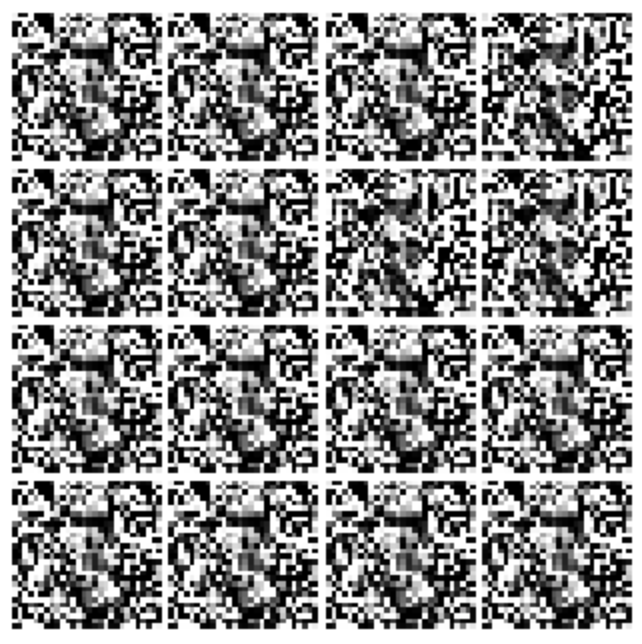
\includegraphics[width=44mm]{latex/WGAN_1e_n10_p1.png} &   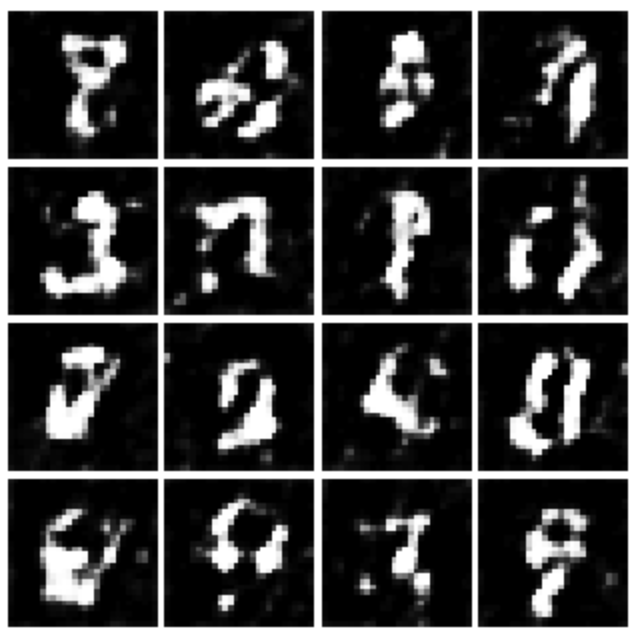
\includegraphics[width=44mm]{latex/WGAN_1e_n10_p001.png} &   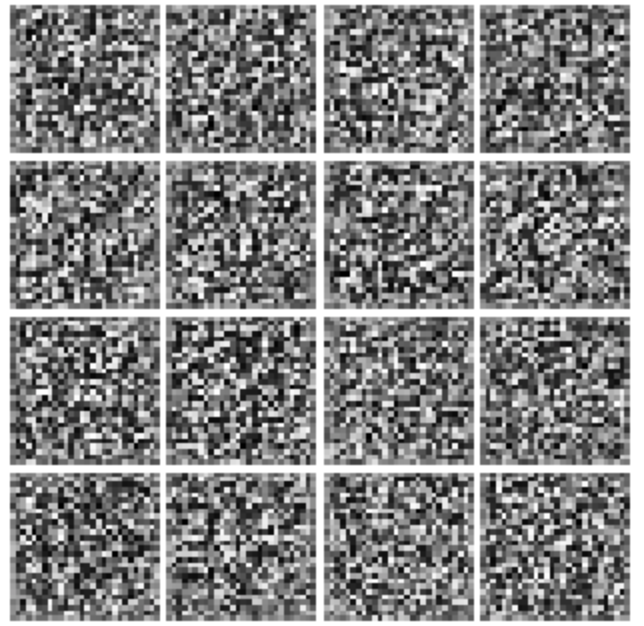
\includegraphics[width=44mm]{latex/WGAN_1e_n10_p00001.png} \\
(g) gradient threshold: $1e-10$ & (h)gradient threshold: $1e-10$& (i)  gradient threshold: $1e-10$\\[6pt]
(g)weight threshold: 0.1 & (h)weight threshold: 0.001 & (i)weight threshold: 0.00001\\[6pt]
\end{tabular}
\caption{Digit images generated by WGAN with features extracted by Convolutional networks. Different gradient threshold and weight threshold settings are applied.}
\label{gans_conv_hyper_p}
\end{figure*}

\begin{table*}[t]
  \centering
  \begin{tabular}{lcr}
   {\bf Algorithm 1} GAN. k is number of steps to apply to the discriminator. \\
   {\color{black} In the original paper k = 1.}\\ \hline
   {\bf for} number of training iterations {\bf do}\\
   \hspace{4mm} {\bf for} k steps {\bf do}\\
   \hspace{8mm} Sample minibatch of $m$ noise samples ${z^{(1)}, ..., z^{(m)}}$ from noise prior $p_g(z)$\\
   % $p_g(z)$\\
   \hspace{8mm} Sample minibatch of $m$ image samples ${x^{(1)}, ..., x^{(m)}}$ from data generating distribution $\mathbb{P}_r(x)$\\
   \hspace{8mm} Update the discriminator with chosen optimizer using gradient: \\
   \hspace{16mm} $\nabla_{\theta_d} \frac{1}{m} \Sigma_{i=1}^m [\log D(x^{(i)}) + \log (1 - D(G(z^{(i)})))]$ \\
   \hspace{4mm} {\bf end for} \\
   \hspace{4mm} Sample minibatch of $m$ noise samples ${z^{(1)}, ..., z^{(m)}}$ from noise prior $p_g(z)$\\
   \hspace{4mm} Update the discriminator with chosen optimizer using gradient: \\
   \hspace{16mm} $\nabla_{\theta_g} \frac{1}{m} \Sigma_{i=1}^m \log (1 - D(G(z^{(i)})))$ \\   
   {\bf end for} \\ \hline
  \end{tabular}
  \label{algo_gan}
\end{table*}


\begin{table*}[t]
  \centering
  \begin{tabular}{lcr}
   {\bf Algorithm 2} WGAN. k is number of steps to apply to the discriminator and c is weight clipping threshold. \\
   {\color{blue} In the original paper k = 5 and c = 0.01.} \\ \hline
   {\bf for} number of training iterations {\bf do}\\
   \hspace{4mm} {\bf for} k steps {\bf do}\\
   \hspace{8mm} Sample minibatch of $m$ noise samples ${z^{(1)}, ..., z^{(m)}}$ from noise prior $p_g(z)$\\
   \hspace{8mm} Sample minibatch of $m$ image samples ${x^{(1)}, ..., x^{(m)}}$ from data generating distribution $\mathbb{P}_r(x)$\\
   % $p_{data}(x)$\\
   \hspace{8mm} Update the discriminator with chosen optimizer using gradient: \\
   \hspace{16mm} {\color{blue} $\nabla_{w} [\frac{1}{m} \Sigma_{i=1}^m f_w(x^{(i)}) + \frac{1}{m} \Sigma_{i=1}^m  f_w(g_\theta(z^{(i)}))]$} \\
   \hspace{16mm} {\color{blue} w $\xleftarrow{}$ clip(w, -c, c)}\\
   \hspace{4mm} {\bf end for} \\
   \hspace{4mm} Sample minibatch of $m$ noise samples ${z^{(1)}, ..., z^{(m)}}$ from noise prior $p_g(z)$\\
   \hspace{4mm} Update the discriminator with chosen optimizer using gradient: \\
   \hspace{16mm} {\color{blue} $\nabla_{\theta} \frac{1}{m} \Sigma_{i=1}^m f_w(g_\theta(z^{(i)}))$ }\\   
   {\bf end for} \\ \hline
  \end{tabular}
  \label{algo_wgan}
\end{table*}


\begin{table*}[t]
  \centering
  \begin{tabular}{lcr}
   {\bf Algorithm 3} $f$-GAN. k is number of steps to apply to the discriminator. \\
   {\color{black} In the original paper k = 1.} \\ \hline
   {\bf for} number of training iterations {\bf do}\\
   \hspace{4mm} {\bf for} k steps {\bf do}\\
   \hspace{8mm} Sample minibatch of $m$ noise samples ${z^{(1)}, ..., z^{(m)}}$ from noise prior $p_g(z)$\\
   \hspace{8mm} Sample minibatch of $m$ image samples ${x^{(1)}, ..., x^{(m)}}$ from data generating distribution $\mathbb{P}_r(x)$\\
   % $p_{data}(x)$\\
   \hspace{8mm} {\color{red} Apply $g_f$ as final layer activation function. For Pearson $\chi^2$ it is identical function.} \\
   \hspace{8mm} Update the discriminator with chosen optimizer using gradient: \\
   \hspace{16mm} {\color{red} $\nabla_{w} [\frac{1}{m} \Sigma_{i=1}^m g_f(V_w(x^{(i)})) - \frac{1}{m} \Sigma_{i=1}^m f^*(g_f(V_w(z^{(i)})))]$, which for Pearson $\Chi^2$ is:}\\
   \hspace{16mm} {\color{red} $\nabla_{w} [\frac{1}{m} \Sigma_{i=1}^m V_w(x^{(i)}) + \frac{1}{m} \Sigma_{i=1}^m \left( \frac{1}{4} V_w(z^{(i)})^2 + V_w(z^{(i)})\right)]$}\\
   % \hspace{16mm} {\color{blue} w $\xleftarrow{}$ clip(w, -c, c)}\\
   \hspace{4mm} {\bf end for} \\
   \hspace{4mm} Sample minibatch of $m$ noise samples ${z^{(1)}, ..., z^{(m)}}$ from noise prior $p_g(z)$\\
   \hspace{4mm} Update the discriminator with chosen optimizer using gradient: \\
   \hspace{16mm} {\color{red} $\nabla_{w} [\frac{1}{m} \Sigma_{i=1}^m f^*(g_f(V_w(z^{(i)})))]$, which for Pearson $\Chi^2$ is:}\\
   \hspace{16mm} {\color{red} $\nabla_{w} [ - \frac{1}{m} \Sigma_{i=1}^m \left( \frac{1}{4} V_w(z^{(i)})^2 + V_w(z^{(i)})\right)]$}\\
   % \hspace{16mm} {\color{blue} w $\xleftarrow{}$ clip(w, -c, c)}\\  
   {\bf end for} \\ \hline
  \end{tabular}
  \label{algo_fgan}
\end{table*}

%-------------------------------------------------------------------------

{\small
\bibliographystyle{ieee}
\bibliography{egbib}
}

\end{document}
